\section{Evaluation On Candidate Selection}

In this section, we discuss how we evaluate Sonda on the context of candidate selection and discuss about the results. Our system Sonda was implemented in Ruby and the queries were implemented as SPARQL queries issues over alive SPARQL endpoints. Sonda is available for download at GitHub as a command line tool $\footnote{https://github.com/samuraraujo/ICDE2013}$, as well as all the results that we obtained. 
 
\subsection{Datasets} 

We evaluated our framework using the datasets and ground truth published by the instance-matching benchmark of the Ontology Alignment
Evaluation Initiative (OAEI) \cite{DBLP:journals/jods/EuzenatMSSS11}. We used the datasets provided in 2010 and 2011. We used the life science (LS) collection (which
includes Sider, Drugbank, Dailymed TCM, and Diseasome) and the Person-Restaurant (PR) from the 2010 collection. We excluded LinkedCT from our experiments due to known quality problem in the ground truth. We used all datasets from the 2011 collection. 

\subsection{Evaluation metrics and alternative approaches} 

We used standard metrics, namely Reduction Ratio (RR), Pair-wise Completeness (PP) and F1. Basically, high RR means that the candidate selection algorithm helps to focus on a smaller number of candidates, while high PP means that it could preserve more of the correct candidates. Because the number of all possible candidates is large in this scenario, we use a normalized version of RR. In particular, these metrics are computed as follows: 
\[
\scriptsize\tt
 PC = \frac{\text{ \#Correctly Computed Candidates}} { \text{ \#Ground Truth Candidates}}
\] 
 \[
 \scriptsize\tt
 RR = \frac{\text{\#Instances with Non-Empty Candidate Sets} }{ \text{\#All Computed Candidates} }
\]

\[
\scriptsize\tt
F1 = \frac{2 * RR * PC}{ RR + PC}
\]
Beside these metrics, we also count the average number of queries evaluated per instance as well as overall time for accomplishing the task of leaning the candidate selection scheme and finding(searching) the candidate sets. 

For comparison, we implemented the \emph{S-agnostic}~\cite{papadakis_efficient_2011} and \emph{S-based}~\cite{DBLP:conf/semweb/SongH11} approaches as discussed in Sec.~2. S-based uses only an OR query and it does not feature the branch-and-bound optimization. It requires key pairs, which are generated as in Sec.~3.1. Further, S-based applies a similarity function on the keys to further prune incorrect candidates after that have been retrieved using the OR queries. For comparison purposes, we apply this strategy to all approaches, using the same similarity function. Sonda uses four types of queries for each key pair, and employs the proposed branch-and-bound optimization to select best queries. 
%. We evaluated our approach with all functionalities that we described before (including the predictor , sorting by time, etc.).

\subsection{Querying Candidates} 
We implemented the queries in our algorithm as SPARQL queries (as discussed before) and directly query a SPARQL endpoint to obtain results (limit to 30 instances per query). For that, we loaded all datasets into the OpenLink Virtuoso Universal Server (Version 6.1.5.3127), except for DBPedia, which we queried its on-line sparql endpoint. We use the default S-P-O index created by this server, and created an inverted index for literal values using the following commands:

\lstset{basicstyle=\small}
\begin{lstlisting}[ ]   
DB.DBA.RDF_OBJ_FT_RULE_ADD 
(null, null, 'index_local');
DB.DBA.VT_INC_INDEX_DB_DBA_RDF_OBJ (); 
\end{lstlisting}

We use the specific Virtuoso SPARQL implementation to have access to the index, and we limited all query results to 30 instances. This avoids the queries to retrieve too many data for non-discriminative queries.

\subsection{Candidate Selection Results} 
Table 1 shows the results. Comparing all approaches over all the 18 datasets pairs that we evaluated, Sonda achieves the best F1 score in 16 cases (in 89\% of the cases, to be precise).
\begin{center}
\begin{table*}[h]
\centering
\scriptsize\tt
\caption{Results of the three systems over all pairs of datasets. Queries denote the total number of queries given to the system. Queries/Instance(Q/I) denotes the amount of queries evaluated per instance.} 
    \begin{tabular}{|c|l|c|c|c|c|c|c|c|c|c|}
        \hline
        Dataset Pairs & Systems & Queries & Q/I & Learning(s) & Search(s)  & RR($\%$) & PC($\%$) &  F1($\%$) \\ \hline

\multirow{4}{*}{DAILYMED-SIDER}  & SondaA  & 40 & 1.63   & 27.73  & 220.04 & 100.0 & 97.86 & 98.92  \\
 & SondaC  & 40 & 1.88   & 29.55  & 228.25 & 100.0 & 98.43 & 99.21  \\
 & S-based  & 8 & 8.0   & 25.17  & 1157.67 & 99.37 & 97.99 & 98.67  \\
 & S-agnostic  & 4 & 4.0   & 15.17  & 638.2 & 99.37 & 97.99 & 98.67  \\ \hline
\multirow{4}{*}{DISEASOME-SIDER}  & SondaA  & 20 & 2.77   & 7.62  & 16.31 & 100.0 & 94.77 & 97.31  \\
 & SondaC  & 20 & 2.47   & 8.54  & 13.97 & 100.0 & 94.77 & 97.31  \\
 & S-based  & 4 & 4.0   & 5.98  & 49.54 & 99.38 & 92.44 & 95.78  \\
 & S-agnostic  & 2 & 2.0   & 2.01  & 27.04 & 100.0 & 91.86 & 95.76  \\ \hline
\multirow{4}{*}{DRUGBANK-SIDER}  & SondaA  & 40 & 1.49   & 56.79  & 36.39 & 100.0 & 99.65 & 99.82  \\
 & SondaC  & 80 & 7.16   & 56.76  & 154.87 & 100.0 & 98.23 & 99.11  \\
 & S-based  & 8 & 8.0   & 50.78  & 265.46 & 95.92 & 99.65 & 97.75  \\
 & S-agnostic  & 29 & 29.0   & 25.2  & 249.16 & 95.59 & 99.65 & 97.58  \\ \hline
\multirow{4}{*}{NYTIMES-DBPEDIA-CORP}  & SondaA  & 15 & 3.28   & 204.11  & 1906.57 & 47.6 & 91.3 & 62.57  \\
 & SondaC  & 30 & 3.33   & 159.5  & 4116.37 & 87.63 & 88.96 & 88.29  \\
 & S-based  & 3 & 3.0   & 106.87  & 1809.11 & 41.04 & 56.39 & 47.51  \\
 & S-agnostic  & 4 & 4.0   & 18.11  & 1771.86 & 13.93 & 33.54 & 19.68  \\ \hline
\multirow{4}{*}{NYTIMES-DBPEDIA-GEO}  & SondaA  & 15 & 3.2   & 319.49  & 2813.14 & 22.76 & 81.09 & 35.54  \\
 & SondaC  & 15 & 1.33   & 143.22  & 521.57 & 62.52 & 75.52 & 68.41  \\
 & S-based  & 3 & 3.0   & 526.5  & 2288.21 & 22.72 & 42.66 & 29.65  \\
 & S-agnostic  & 5 & 5.0   & 10.22  & 2769.9 & 6.26 & 31.35 & 10.44  \\ \hline
\multirow{4}{*}{NYTIMES-FREEBASE-CORP}  & SondaA  & 15 & 1.68   & 37.81  & 489.66 & 98.88 & 87.88 & 93.06  \\
 & SondaC  & 45 & 2.92   & 42.85  & 641.44 & 99.24 & 89.85 & 94.31  \\
 & S-based  & 3 & 3.0   & 23.66  & 1262.01 & 86.6 & 69.97 & 77.4  \\
 & S-agnostic  & 4 & 4.0   & 13.03  & 588.26 & 81.1 & 42.35 & 55.64  \\ \hline
\multirow{4}{*}{NYTIMES-FREEBASE-GEO}  & SondaA  & 15 & 2.57   & 37.79  & 621.28 & 97.62 & 87.71 & 92.4  \\
 & SondaC  & 15 & 2.29   & 36.32  & 597.06 & 97.56 & 88.13 & 92.6  \\
 & S-based  & 3 & 3.0   & 31.13  & 866.07 & 79.88 & 56.51 & 66.19  \\
 & S-agnostic  & 5 & 5.0   & 12.35  & 498.78 & 78.11 & 45.78 & 57.73  \\ \hline
\multirow{4}{*}{NYTIMES-FREEBASE-PER}  & SondaA  & 15 & 2.1   & 42.28  & 1153.96 & 95.49 & 95.58 & 95.54  \\
 & SondaC  & 30 & 3.09   & 43.58  & 1348.91 & 93.7 & 96.04 & 94.86  \\
 & S-based  & 3 & 3.0   & 38.07  & 3180.94 & 93.63 & 73.55 & 82.39  \\
 & S-agnostic  & 4 & 4.0   & 25.06  & 1216.74 & 95.32 & 29.54 & 45.11  \\ \hline
\multirow{4}{*}{NYTIMES-GEONAMES}  & SondaA  & 15 & 3.33   & 129.97  & 1826.46 & 16.19 & 90.5 & 27.47  \\
 & SondaC  & 15 & 3.33   & 128.32  & 2024.58 & 16.19 & 90.5 & 27.47  \\
 & S-based  & 3 & 3.0   & 38.85  & 1194.26 & 27.54 & 23.59 & 25.41  \\
 & S-agnostic  & 5 & 5.0   & 11.2  & 552.14 & 28.45 & 19.62 & 23.23  \\ \hline
\multirow{4}{*}{PERSON11-PERSON12}  & SondaA  & 15 & 1.27   & 11.17  & 26.69 & 99.57 & 95.63 & 97.56  \\
 & SondaC  & 15 & 1.26   & 11.18  & 26.95 & 99.57 & 95.63 & 97.56  \\
 & S-based  & 3 & 3.0   & 9.0  & 62.76 & 78.68 & 96.25 & 86.58  \\
 & S-agnostic  & 4 & 4.0   & 4.46  & 68.34 & 30.98 & 100.0 & 47.3  \\ \hline
\multirow{4}{*}{PERSON21-PERSON22}  & SondaA  & 20 & 7.16   & 5.91  & 20.19 & 44.59 & 58.47 & 50.6  \\
 & SondaC  & 20 & 6.24   & 5.91  & 18.23 & 44.3 & 59.32 & 50.72  \\
 & S-based  & 4 & 4.0   & 4.29  & 13.64 & 25.19 & 87.29 & 39.09  \\
 & S-agnostic  & 4 & 4.0   & 0.54  & 11.07 & 21.88 & 100.0 & 35.9  \\ \hline
\multirow{4}{*}{RESTAURANT1-RESTAURANT2}  & SondaA  & 10 & 1.83   & 5.14  & 8.37 & 98.25 & 98.23 & 98.24  \\
 & SondaC  & 10 & 1.82   & 5.06  & 8.12 & 98.25 & 98.23 & 98.24  \\
 & S-based  & 2 & 2.0   & 3.42  & 18.81 & 94.02 & 96.46 & 95.22  \\
 & S-agnostic  & 3 & 3.0   & 0.74  & 17.93 & 94.02 & 96.46 & 95.22  \\ \hline
\multirow{4}{*}{SIDER-DAILYMED}  & SondaA  & 35 & 3.88   & 177.38  & 140.55 & 34.96 & 64.67 & 45.38  \\
 & SondaC  & 105 & 11.55   & 179.45  & 315.42 & 40.33 & 57.07 & 47.26  \\
 & S-based  & 7 & 7.0   & 173.95  & 583.63 & 25.05 & 83.83 & 38.57  \\
 & S-agnostic  & 3 & 3.0   & 32.61  & 7781.31 & 36.02 & 75.63 & 48.8  \\ \hline
\multirow{4}{*}{SIDER-DBPEDIA-DRUGS}  & SondaA  & 10 & 1.52   & 46.05  & 112.57 & 98.06 & 92.1 & 94.99  \\
 & SondaC  & 30 & 2.28   & 41.36  & 199.11 & 99.72 & 94.69 & 97.14  \\
 & S-based  & 2 & 2.0   & 39.27  & 145.72 & 77.56 & 93.04 & 84.6  \\
 & S-agnostic  & 3 & 3.0   & 35.41  & 155.64 & 69.18 & 93.19 & 79.41  \\ \hline
\multirow{4}{*}{SIDER-DBPEDIA-SIDEEFFECT}  & SondaA  & 20 & 1.58   & 33.43  & 303.39 & 76.69 & 89.29 & 82.51  \\
 & SondaC  & 40 & 4.66   & 21.21  & 508.37 & 94.44 & 90.58 & 92.47  \\
 & S-based  & 4 & 4.0   & 23.86  & 543.29 & 77.42 & 71.74 & 74.47  \\
 & S-agnostic  & 3 & 3.0   & 4.51  & 400.67 & 56.85 & 65.42 & 60.83  \\ \hline
\multirow{4}{*}{SIDER-DISEASOME}  & SondaA  & 20 & 4.52   & 10.05  & 43.41 & 83.33 & 94.77 & 88.68  \\
 & SondaC  & 20 & 4.53   & 9.82  & 47.45 & 83.33 & 94.77 & 88.68  \\
 & S-based  & 4 & 4.0   & 7.64  & 91.51 & 86.19 & 91.86 & 88.93  \\
 & S-agnostic  & 3 & 3.0   & 1.27  & 47.1 & 90.17 & 88.95 & 89.56  \\ \hline
\multirow{4}{*}{SIDER-DRUGBANK}  & SondaA  & 25 & 3.59   & 52.65  & 269.51 & 95.67 & 98.02 & 96.83  \\
 & SondaC  & 25 & 2.38   & 54.81  & 153.76 & 98.25 & 97.44 & 97.84  \\
 & S-based  & 5 & 5.0   & 50.27  & 470.65 & 94.22 & 99.3 & 96.69  \\
 & S-agnostic  & 3 & 3.0   & 41.43  & 337.92 & 97.11 & 97.79 & 97.45  \\ \hline
\multirow{4}{*}{SIDER-TCM}  & SondaA  & 10 & 1.68   & 7.8  & 14.0 & 100.0 & 98.25 & 99.12  \\
 & SondaC  & 10 & 1.61   & 7.75  & 12.48 & 100.0 & 98.25 & 99.12  \\
 & S-based  & 2 & 2.0   & 4.85  & 22.8 & 100.0 & 95.32 & 97.6  \\
 & S-agnostic  & 3 & 3.0   & 1.17  & 24.21 & 100.0 & 95.32 & 97.6  \\ \hline	
 \multirow{4}{*}{Average}  & SondaA  &  19.72	& 2.73 & 	67.40 & 	556.81 & 	78.31 & 	89.77 & 	80.92\\
 & SondaC  & 31.39	& 3.56 &	54.73 & 	607.61	& 84.17	& 89.25 & 	85.03 \\
 & S-based  & 3.94	& 3.94	& 	64.64	& 	779.23	& 	72.47	& 	79.32	& 	73.47\\
  & S-agnostic  & 5.06 &  	5.06	 & 14.14 & 	953.13	 & 66.35	 & 72.47 & 	64.22\\ \hline	
 
\end{tabular}  
\end{table*} 
\end{center}

\textbf{Data Ambiguity}. Sonda ($Sonda_A$ and $Sonda_C$) was much more effective (F1) than other approaches when data was more ambiguous  (e.g., Freebase, DBPedia and Geonames cases), achieving a considerable improvement in both RR and PC than the other approaches. Mainly, those approaches performed worse because they considered only OR queries (that are too inclusive and penalize RR),  and as a query limit was used in all queries, it also decrease the PC, due to the correct matches were out of the sets defined by those limits. As S-agnostic has the most inclusive type of queries, it had the worse performance (F1) in those cases, penalizing even more PC.

\textbf{Class Queries}. The RR in $Sonda_C$ was considerably higher than in $Sonda_A$ for a few cases (DBPedia, Freebase and Geonames). This occurred due to class level ambiguity (many instances with the same name but from different classes) in those datasets. It indicates that the class clauses indeed make the queries more precise because it select exactly the correct class of target instances. However, an increase on searching time can be observed in $Sonda_C$, mainly due to a higher number of queries that were considered in this version.

\textbf{Time Performance and F1-Measure}. Regarding the learning time performance, in average it takes less than 10\% of the overall searching time. Although, a more complex learning process (that produces better comparable keys) takes more time, it leads to a better F1. 

In general, the best F1 can only be achieved by using an complex learning process and an efficient execution process. For instance, S-based used the same set of comparable keys than Sonda, but it achieved the worse searching time performance in all cases. Even though Sonda has more queries to evaluate (because it uses different types of queries with different time performances), it is faster than S-based, because its  branch-and-bound algorithm helps to select the ones that require less evaluation time (those that are more efficient than the ones used by the other approaches).  In average, S-agnostic has the best learning and searching time performance, but the worse F1. 

Concluding, the best F1 is associated to learn effective comparable keys, which take more time to compute, and to learn efficient queries execution plan, which can efficiently execute the most effective queries. 
 
 
 \textbf{Query Type Performance}.  Although the 
 Fig. \ref{fig:time} shows the evaluation time per query type. It confirms our intuition that EXACTLANG and EXACT are the fastest one; however, they are not optimal in many cases, as observed in Fig. \ref{fig:frequency}, which shows the frequency that the queries types were consider optimal per dataset. This diagram reinforces that there is no one type of query that are optimal for all cases; therefore, a smart choice of a template query per each instance by optimization the search space is really necessary. 
 \begin{figure} [h]
\vspace{-10pt}
\centering
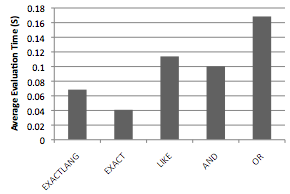
\includegraphics[scale=0.5]{p9.png}
\caption{Average evaluation time of the query types.} 
\vspace{-10pt}
\label{fig:time}
\end{figure} 

 \begin{figure} [h]
\vspace{-10pt}
\centering
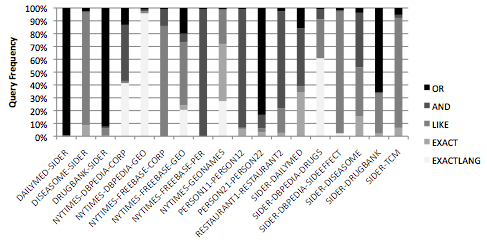
\includegraphics[scale=0.5]{p8.png}
\caption{Frequency in which the query types were consider optimal on SondaA.} 
\vspace{-10pt}
\label{fig:frequency}
\end{figure}


\textbf{Query Type Effectiveness}. As S-based and S-agnostic considered more inclusive queries (OR queries) than Sonda, we can conclude that, although necessary, more inclusive queries leads to worse F1, mainly because they decrease the RR, and as it was used a limit on queries, it also decrease the PC. 



\textbf{Predictor and Branching Policy Efficiency}. We can see that in all cases, Sonda achieves a considerable reduction in the number of queries evaluated per instance. In some cases (e.g., Dailymed-Sider, Diseasome-Sider), it performed nearly one query per instance. Notice that we can not compare the predictor on S-based and S-agnostic, because in both cases, the number of queries executed per instance is fixed. The purpose here is to show  that Sonda's predictor and branching policy was very efficient, selecting only a few queries per instance, as well as, very effective, selecting queries that produce near optimal PC, in many cases. 


\begin{center}
\begin{table*}[h]
\centering
\scriptsize\tt
\caption{Sonda F1-measure (between precision and recall) compared to ExampleDriven and other tools that participate on the OAEI 2011 benchmark.} 
\begin{tabular}{|c|c|c|c|c|c|c|c|}
\hline
Dataset  &  SondaA  &  SondaC & KnoFuss+GA & AggreementMaker & SERIMI & Zhishi.links & ExampleDriven\\ \hline
DBPedia - Geo. & 0.63 & 0.63  & 0.89 & 0.69 & 0.68 & 0.92 & 0 \\ \hline
DBPedia - Corp. & 0.91 & 0.91 & 0.92 & 0.74 & 0.88 & 0.91 & 0\\ \hline
DBPedia - People & 0.96 & 0.96 & 0.97 & 0.88 & 0.94 & 0.97 & 0\\ \hline
Freebase - Geo. & 0.90 & 0.90 & 0.93 & 0.85 & 0.91 & 0.88 & 0\\ \hline
Freebase - Corp. & 0.87 & 0.87 & 0.92 & 0.80 & 0.91 & 0.87 & 0\\ \hline
Freebase - People & 0.96 &  0.96 & 0.95 & 0.96 & 0.92 & 0.93 & 0\\ \hline
Geonames & 0.63 & 0.63  & 0.90 & 0.85 & 0.80 & 0.91 & 0\\ \hline
Average & 0 & 0  & 0.93 & 0.85 & 0.89 &  0.92 & 0\\ \hline											 
\end{tabular}  
\end{table*} 
\end{center}

\begin{center}
\begin{table*}[h]
\centering
\scriptsize\tt
\caption{Sonda  F1-measure (between precision and recall) compared ExampleDriven and  other tools that participate on the OAEI 2010 benchmark.} 
\begin{tabular}{|c|c|c|c|c|c|c|}
\hline
Dataset &  $Sonda_A$ & $Sonda_C$& SERIMI & ObjectCoref & Rimon & ExampleDriven \\ \hline
Sider-Dailymed & 0.63 & 0.61   & \textbf{0.66} & - & 0.62  & 0\\ \hline
Sider-Diseasome & \textbf{0.90} & 0.90   & 0.87 & - & 0.45 & 0\\ \hline
Sider-Drugbank & 0.93 & 0.93  & \textbf{0.97} & - & 0.50  & 0\\ \hline
Sider-TCM & 0.92 & 0.92  & \textbf{0.97} & - & 0.79 &  0\\ \hline
Dailymed-Sider & 0.93  &\textbf{0.94} & 0.67 & 0.70 & 0.62  & 0\\ \hline
Drugbank-Sider & \textbf{0.80}  & \textbf{0.80} & 0.48 & 0.46 & -  & 0\\ \hline
Diseasome-Sider & \textbf{0.95} & \textbf{0.95}  & 0.87 & 0.74 & -  & 0\\ \hline
Person11-Person12 & 0.95 & 0.95  & \textbf{1.00} & 0.99 & \textbf{1.00}  & 0\\ \hline
Person21-Person22 & 0.45 & 0.45  & 0.46 & 0.95 & \textbf{0.97} & 0\\ \hline
Restaurant1-Restaurant2 & \textbf{0.98} & \textbf{0.98}  & 0.77 & 0.81  & 0.88 & 0\\ \hline
Average\footnote{Average of all datasets} &  		\textbf{0.84}	& \textbf{0.84}	& 0.77 & - & - &0						 	\\ \hline								 
Average\footnote{Average of datasets evaluated by Objecoref} &  	0.84 &	\textbf{0.85}	&0.71&	0.78&-&0\\ \hline
Average\footnote{Average of datasets evaluated by Rimon} &\textbf{0.84}	&\textbf{0.84}	&0.80	&	-&0.73 & 0\\ \hline
\end{tabular}  
\end{table*} 
\end{center}



\section{Evaluation On Instance Matching}
In this section, we discuss how we evaluate Sonda on the context of instances matching.  Mainly, we apply two matcher overs the candidates sets produced by Sonda. Then, we compared the results of the match with state-of-the-art instance matching approaches that participate on the OAEI 2010 and 2011 challenge. Also, the ExampleDriven approach was evaluated over the same datasets. As evaluation metrics, we used standard precision, recall and F1 metrics. 

\subsection{Instance Matching Results} 

In this section, we compared the Sonda F1-measure (between precision and recall) with the other alternatives approaches that were evaluated over the same datasets.
%Notice that although not ideal, Sonda completed the task in a reasonable time, considering that our approach queried directly the datasets SPARQL endpoints. 
%The drawback of this approach is that there is a huge time delay due to access to disc, packing of the data in the SPARQL protocol and transferring it via the network. In the other hand, we can integrate two alive data endpoint without any configuration issues, parameter tuning, data pre-processing and indexing, in a couple of minutes or in a few hours. 

%In summary, Sonda yields better F1 score in 96\% of the cases and also, . It means Sonda is more effective in selecting the candidates compared to other approaches, and the main reason for that is attributed to the use of multiple query types and the smart selection of the queries by the branch-and-bound algorithm.


 

 